\section{Results}
\label{sec:results}

\para{Main behavioral comparison.}
\Tabref{tab:acc_main} shows near-identical performance between \direct and \cotprompt conditions. \direct is slightly higher (90.0\% vs. 89.2\%), but confidence intervals overlap broadly.

\begin{table}[t]
\centering
\caption{Behavioral accuracy on 120 \csqa validation items. Wilson 95\% confidence intervals are reported. Best accuracy in \textbf{bold}.}
\label{tab:acc_main}
\begin{tabular}{@{}lccc@{}}
\toprule
Method & Accuracy & 95\% CI & N \\
\midrule
\direct & \textbf{0.900} & [0.833, 0.942] & 120 \\
\cotprompt & 0.892 & [0.823, 0.936] & 120 \\
\bottomrule
\end{tabular}
\end{table}

\begin{table}[t]
\centering
\caption{Directional failure flips between conditions.}
\label{tab:flips}
\begin{tabular}{@{}lcc@{}}
\toprule
Flip type & Rate & Count \\
\midrule
\direct correct $\rightarrow$ \cotprompt wrong & 0.0250 & 3 \\
\cotprompt correct $\rightarrow$ \direct wrong & 0.0167 & 2 \\
\bottomrule
\end{tabular}
\end{table}

McNemar exact test on discordant pairs gives $b=3$, $c=2$, $n_{\text{discordant}}=5$, and $p=1.0$, so we do not reject equal paired performance.

\begin{figure}[t]
    \centering
    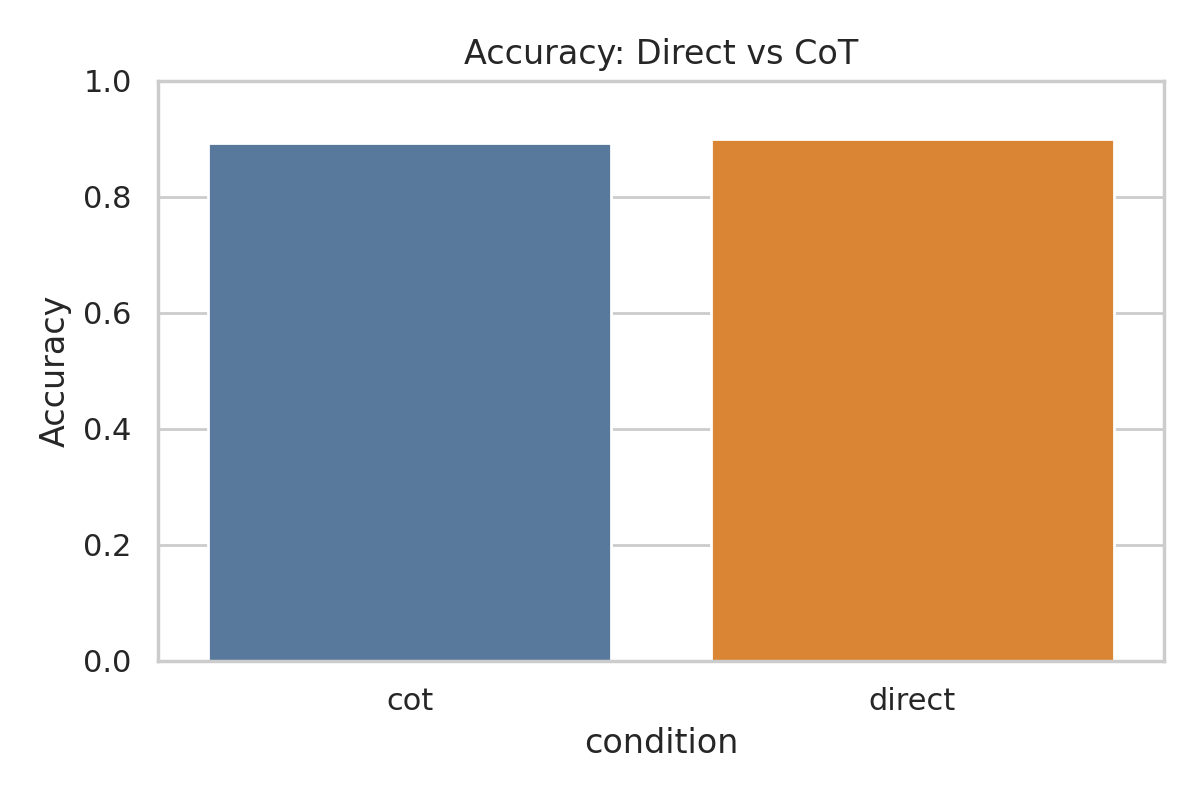
\includegraphics[width=0.95\linewidth]{figures/accuracy_direct_vs_cot.png}
    \caption{Behavioral accuracy comparison between \direct and \cotprompt prompting. Error bars visualize uncertainty intervals and show no practical gap.}
    \label{fig:behavioral_accuracy}
\end{figure}

\para{Coherence scoring.}
Coherence judgments are close to ceiling in most groups, which limits discriminative power for failure diagnosis. \Figref{fig:coherence_rates} illustrates this saturation pattern.

\begin{figure}[t]
    \centering
    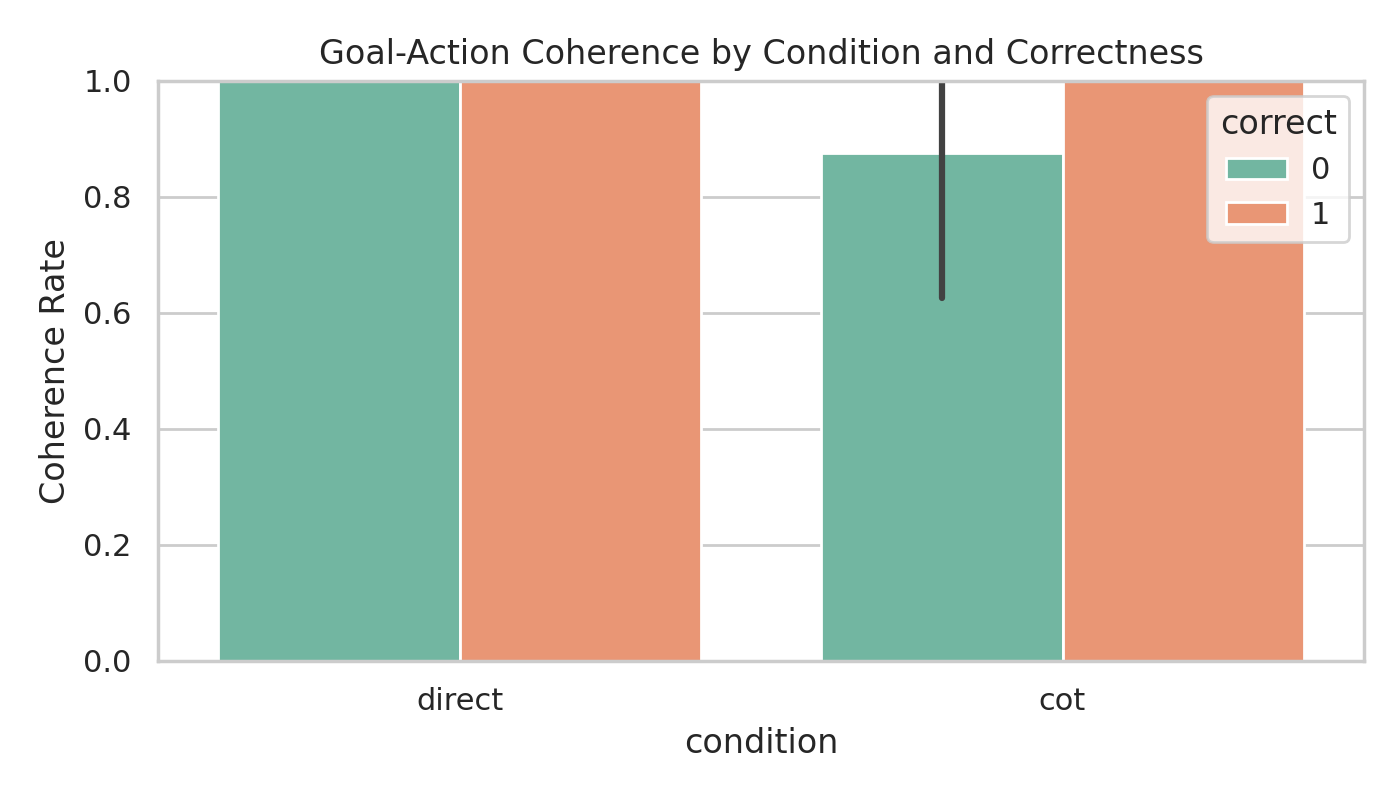
\includegraphics[width=0.95\linewidth]{figures/coherence_rates.png}
    \caption{Goal-action coherence rates by condition and outcome subgroup. Rates cluster near 1.0, indicating a ceiling effect in this judge configuration.}
    \label{fig:coherence_rates}
\end{figure}

\para{Mechanistic proxy intervention results.}
\Tabref{tab:mechanistic} summarizes the layer-ablation proxy test. The target-layer effect is small and not significant by either parametric or nonparametric paired testing.

\begin{table}[t]
\centering
\caption{Mechanistic proxy test on matched success/failure examples in \proxy.}
\label{tab:mechanistic}
\begin{tabular}{@{}lc@{}}
\toprule
Statistic & Value \\
\midrule
Matched examples & 24 \\
Layers scanned & 6 \\
Target layer & 3 \\
Paired $t$-test $p$ & 0.853 \\
Wilcoxon $p$ & 0.546 \\
Cohen's $d$ (paired) & 0.038 \\
\bottomrule
\end{tabular}
\end{table}

\begin{figure}[t]
    \centering
    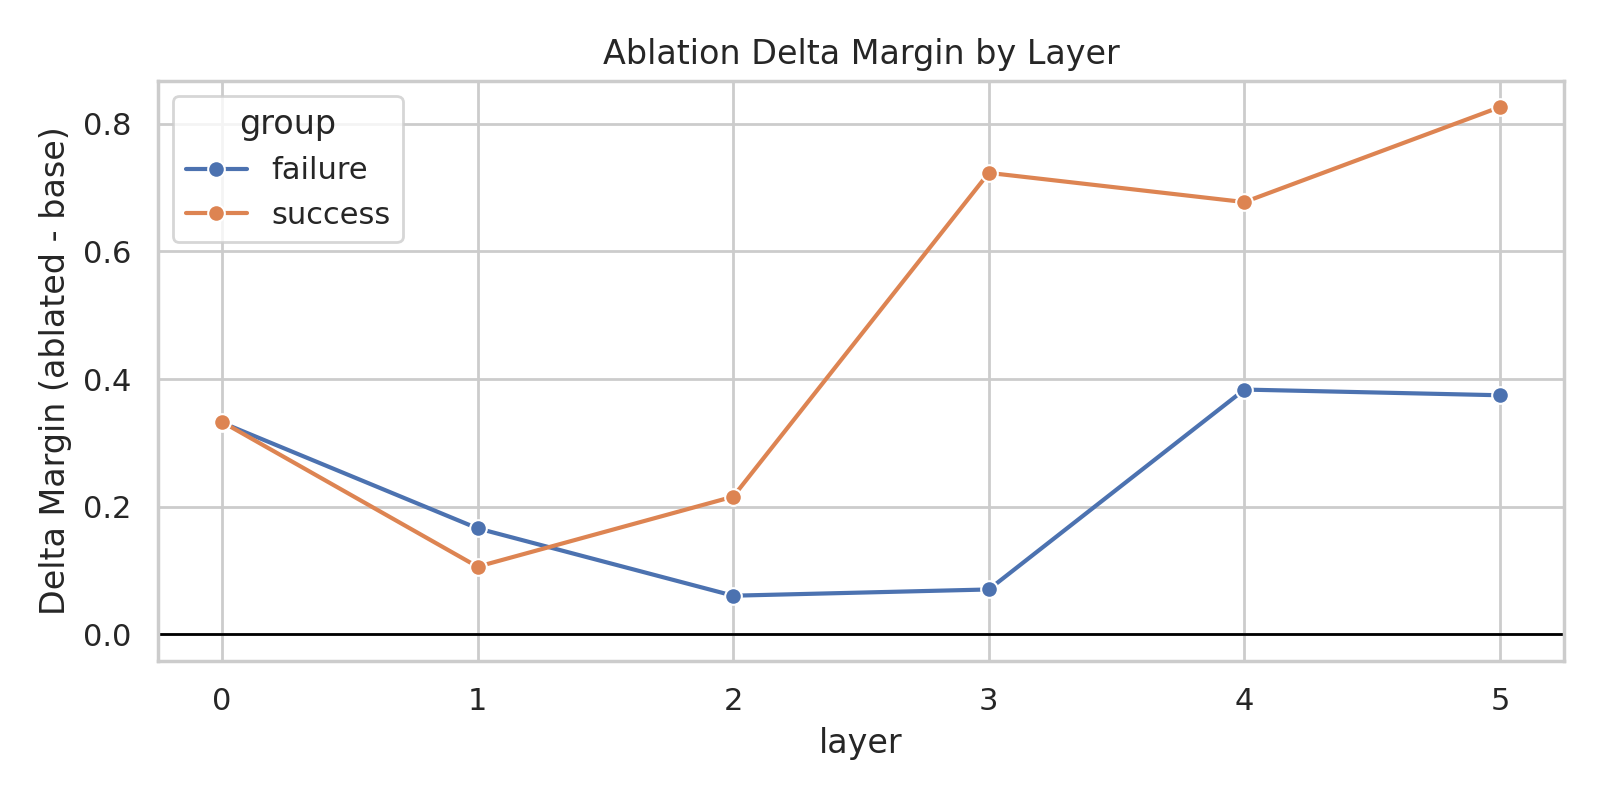
\includegraphics[width=0.95\linewidth]{figures/layer_ablation_deltas.png}
    \caption{Layer-wise ablation deltas in coherent-margin proxy. Variability dominates and no single layer shows a robust directional effect in this small model scan.}
    \label{fig:layer_ablation}
\end{figure}

\para{Ablation interpretation.}
The intervention track is a coarse ablation study at layer granularity. It does not isolate head-level or path-level mechanisms, and the null result should be interpreted as non-localization under this proxy rather than evidence that no mechanism exists.
